\section{Menu flowchart and explanation~\ref{fig:menu}}
\begin{figure}
    \centering 
    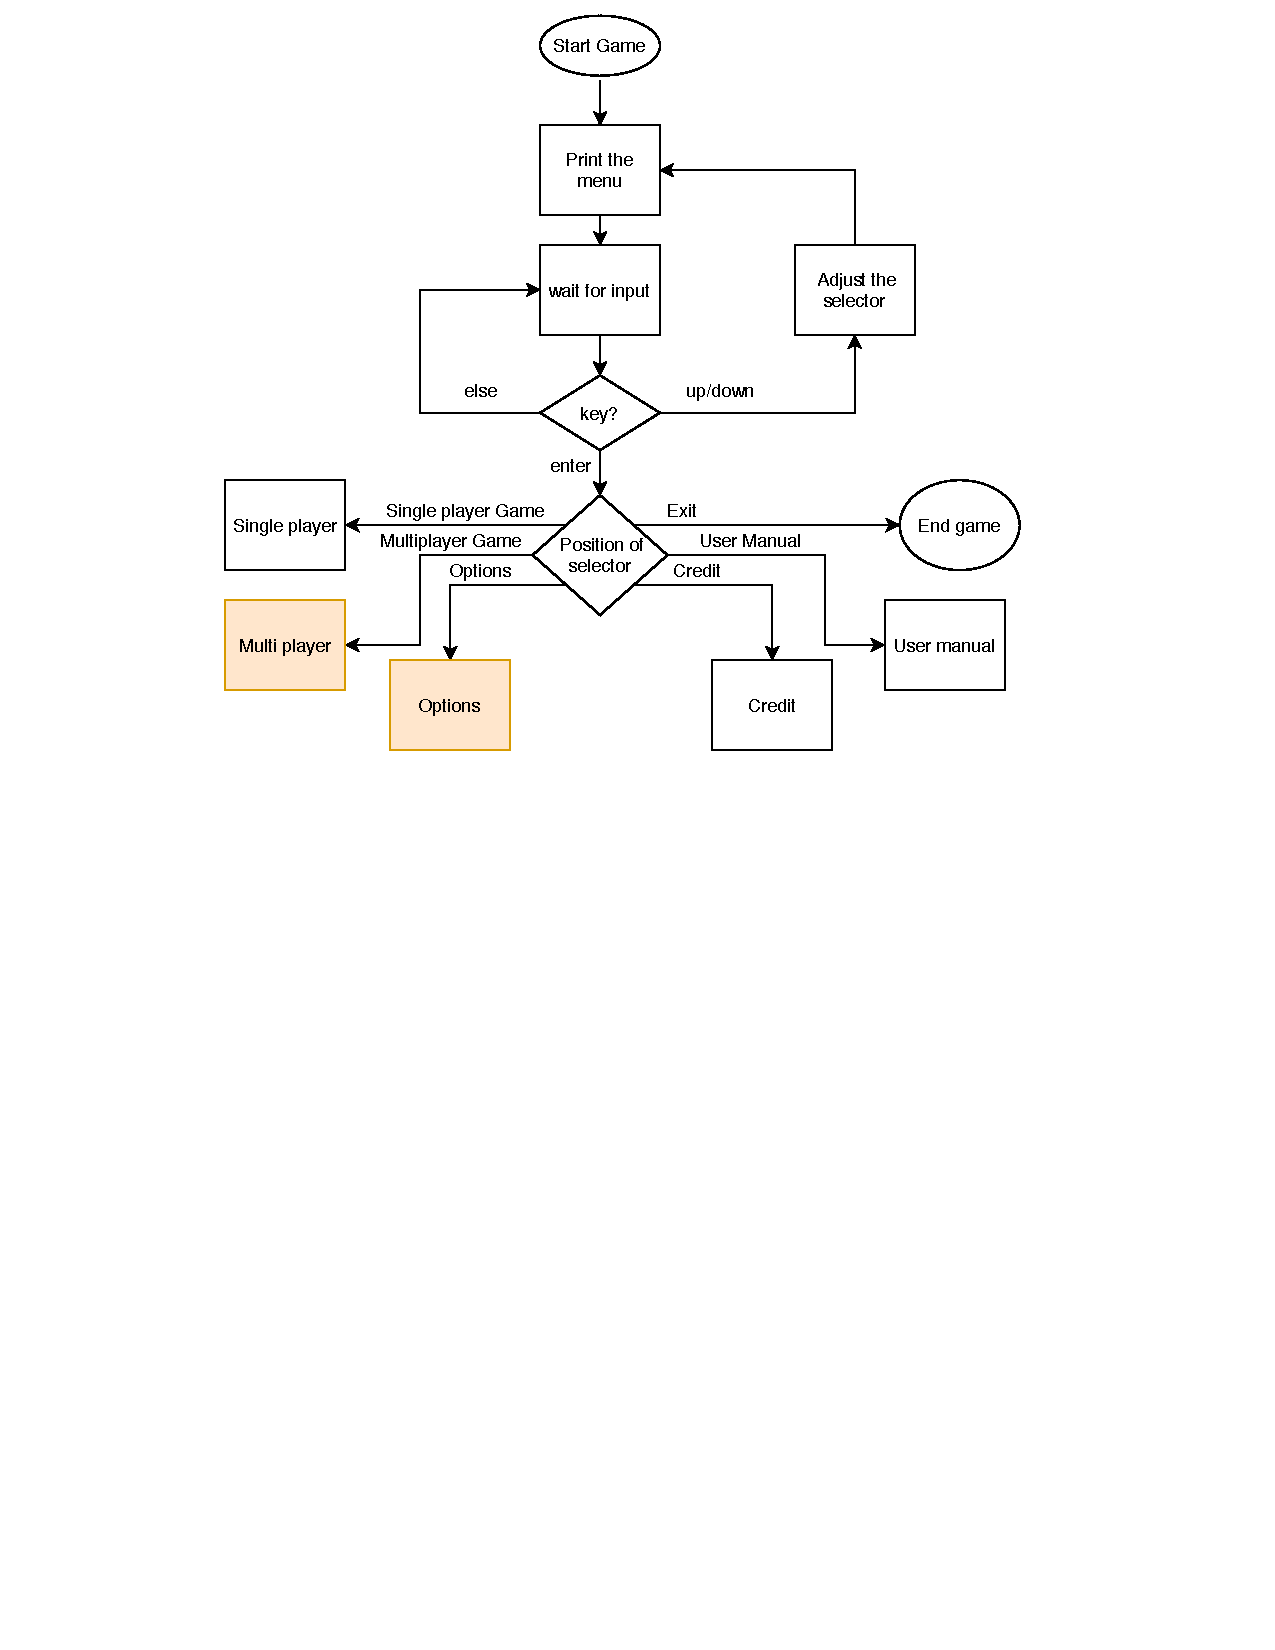
\includegraphics[width=0.8\columnwidth]{menu.pdf}
    \caption{Menu flowchart. white blocks are implemented in first release and \textcolor{orange}{orange} blocks are implemented in second release. }
    \label{fig:menu}
\end{figure}

This section explains the flow of our program since execution starts until it finishes. 
As it is shown in Figure \ref{fig:menu}, initially, we print a menu for the game. There are multiple choices on the game menu and user can go through each of them and press enter to select one. So, program is waiting for the user to press a key.
There is a selector which places besides each menu item. The user can see the selector and be informed on its selection. Adjust the selector block is responsible for this operation.
Next step decides what to do based on the user's choice. 
As we seen in Figure~\ref{fig:menu}, we may go on six different scenarios: user manual, single player, multiplayer, options, credit and end game which will be explained in detail in the coming sections.

\subsection{Menu functions prototype}
In this section we define the required functions prototypes and its relation to flow chart. Comments above each function mention the associated block, the release, and assignee.

\begin{minted}{c}
#define MAX_ITEM_SIZE 100
#define NUM_OF_ITEMS 6

typedef enum {
	USER_MANUAL,
	SINGLE_PLAYER,
	MULTI_PLAYER,
	OPTION,
	CREDIT,
	EXIT,	
} MenuSelector;

typedef struct MenuItem {
	char str[MAX_ITEM_SIZE];
} MenuItem;

typedef struct Menu {
	MenuSelector selector;
	MenuItem items[NUM_OF_ITEMS];
} Menu;

/* Block: Print the menu - first release
 * Assigned to: Jaser
 * Prints the game start up menu on the consol.
 * Input: menu
 * Return: void */
void printMenu(Menu menu);

/* Block: Adjust the selector - first release
 * Assigned to: Jaser
 * Updates the selector position according to input key.
 * Input: menu_p, arrowKey
 * Output: menu_p
 * Return: void */
void updateSelector(Menu* menu_p, int arrowKey);

/* Block: Options - second release
 * Assigned to: Jaser
 * Calls functions related to options
 * Input: void
 * Output: void
 * Return: void*/
void option(void);

/* Block: Single player - first release
 * Assigned to: Pari
 * Calls functions related to Single Player Setup 
 * on Level 2 flowchart
 * Input: void 
 * Output: void
 * Return: void */
void singlePlayer(void);

/* Block: Credit - first release
 * Assigned to: Mahsa
 * shows information about the credit.
 * Input: void 
 * Output: void
 * Return: void */
void credit(void);

/* Block: Multi player - second release
 * Assigned to: Jin
 * Calls functions related to multiplayer setup.
 * Input: void 
 * Output: void
 * Return: void */
void multiPlayer(void);

/* Block: End game - first release
 * Assigned to: Mahsa
 * Exit from the game
 * Input: void 
 * Output: void
 * Return: void */
void exit(void);

/* Block: User manual - first release
 * Assigned to: Jin
 * displays a user manual for the player (how to Play).
 * Input: void 
 * Output: void
 * Return: void */
void userManual(void);
\end{minted}